    %!TEX encoding = UTF-8 Unicode 
\documentclass[usenames,dvipsnames]{beamer}

    \usetheme{metropolis}

   \usecolortheme{seahorse}
   
        \usepackage{pgfpages}
\usepackage{CJKutf8} 
\usepackage{tcolorbox}
\usepackage[textfont={small}]{caption}

    \setbeamercovered{invisible}
    \usepackage{tikz}   
    \usetikzlibrary{shapes,arrows}
\usepackage{graphicx}% http://ctan.org/pkg/graphicx
\usepackage{booktabs}
    \usepackage{framed, color}
    \definecolor{shadecolor}{rgb}{1, 0.8, 0.3}
    % To remove the navigation symbols from
    % the bottom of slides%
 %\setbeameroption{show notes on second screen}
%\setbeameroption{show only notes}
    \setbeamertemplate{navigation symbols}{}
    %
  \setbeamercolor{section in head/foot}{fg=black, bg=structure.fg!20!white}

\usepackage[natbibapa]{apacite}
\bibliographystyle{apacite}
\bibpunct{(}{)}{;}{a}{}{,}

\usetikzlibrary{calc}


\tikzstyle{decision} = [diamond, draw, fill=blue!20, 
    text width=4.5em, text badly centered, node distance=3cm, inner sep=0pt]
\tikzstyle{block} = [rectangle, draw, fill=blue!20, 
    text width=6em, text centered, rounded corners, minimum height=4em]
\tikzstyle{line} = [draw, -latex']
\tikzstyle{cloud} = [draw, ellipse,fill=red!20, node distance=3cm,
    minimum height=2em]

\newcommand{\tikzmark}[1]{\tikz[overlay,remember picture] \node (#1) {};}
\newcommand{\DrawBox}[1][]{%
    \tikz[overlay,remember picture]{
    \draw[red,#1]
      ($(left)+(-0.2em,0.9em)$) rectangle
      ($(right)+(0.2em,-0.3em)$);}
}

\newenvironment{variableblock}[3]{%
  \setbeamercolor{block body}{#2}
  \setbeamercolor{block title}{#3}
  \begin{block}{#1}}{\end{block}}

\makeatletter
\setbeamertemplate{footline}
{
  \leavevmode%
  \hbox{%
  \begin{beamercolorbox}[wd=1\paperwidth,ht=2.25ex,dp=1ex,center]{author in head/foot}%
    \usebeamerfont{author in head/foot}%
    \insertsectionnavigationhorizontal{0.8\paperwidth }{}{}%
     \insertframenumber /  \inserttotalframenumber
 \end{beamercolorbox}}%
 % \begin{beamercolorbox}[wd=.3\paperwidth,ht=2.25ex,dp=1ex,right]{date in head/foot}%
   % \usebeamerfont{date in head/foot}\insertshortdate{}\hspace*{2em}
  \hspace*{2ex} 
  %\end{beamercolorbox}}%
  \vskip0pt%
}


\usepackage{graphicx}
\usepackage[caption=false]{subfig}
\usepackage{multicol}
\usepackage{color, colortbl}
\definecolor{Gray}{gray}{0.9}

%\definecolor{white}{white}{0.9}

%\setbeamercovered{white}
    %\usepackage{bm} % For typesetting bold math (not \mathbold)
    %\logo{\includegraphics[height=0.6cm]{yourlogo.eps}}
\title{Are legislators more responsive to high quality evidence? A field experiment}
\author{Angèle Delevoye and Trevor Incerti}

\date{29 May 2019} 


\begin{document}
\maketitle

%%%%%%%%%%%%%%%%%%%%%%%%%%%%%%%%%%%

\section{Introduction}

\begin{frame}
\frametitle{Research Questions}
\begin{itemize}
\item Do policymakers \textcolor{Cerulean}{give more credence} to high quality research?
\vspace{15mm}
\pause
\item Can policymakers \textcolor{Cerulean}{recognize} differences in research quality?
\end{itemize}
\end{frame}

%\item Heterogeneity by party \hyperlink{hte_party}{\beamerbutton{Figure}} and pre-existing nationalism \hyperlink{hte_nat}{\beamerbutton{Figure}} in Japan. 

%%%%%%%%%%%%%%%%%%%%%%%%%%%%%%%%%%%

\section{Theory}

\begin{frame}
\frametitle{Pre-existing literature}

\begin{itemize}
\item Stuff here
\end{itemize}

\end{frame}

%%%%%%%%%%%%%%%%%%%%%%%%%%%%%%%%%%%

\begin{frame}
\frametitle{Evidence standards}

\begin{itemize}
\item Evidence standards and descriptions already adopted in federal legislation.
\begin{itemize}
\item Secondary Education Act, No Child Left Behind, Every Student Succeeds Act
\end{itemize}
\item Department of Education standards.
\begin{itemize}
\item Strong causal evidence
\item Moderate causal evidence
\item Low causal evidence
\item High levels of specificity, covering IVs, cluster-random assignment, RDs, and missingness/attrition. 
\end{itemize}
\item Department of Labor has adopted similar standards \hyperlink{doe_evidence}{\beamerbutton{Figure}}
\end{itemize}

\end{frame}

%%%%%%%%%%%%%%%%%%%%%%%%%%%%%%%%%%%

\begin{frame}
\frametitle{DoE evidence standards}

\begin{center}
\vspace{-0.85cm}
\hspace*{-1cm}
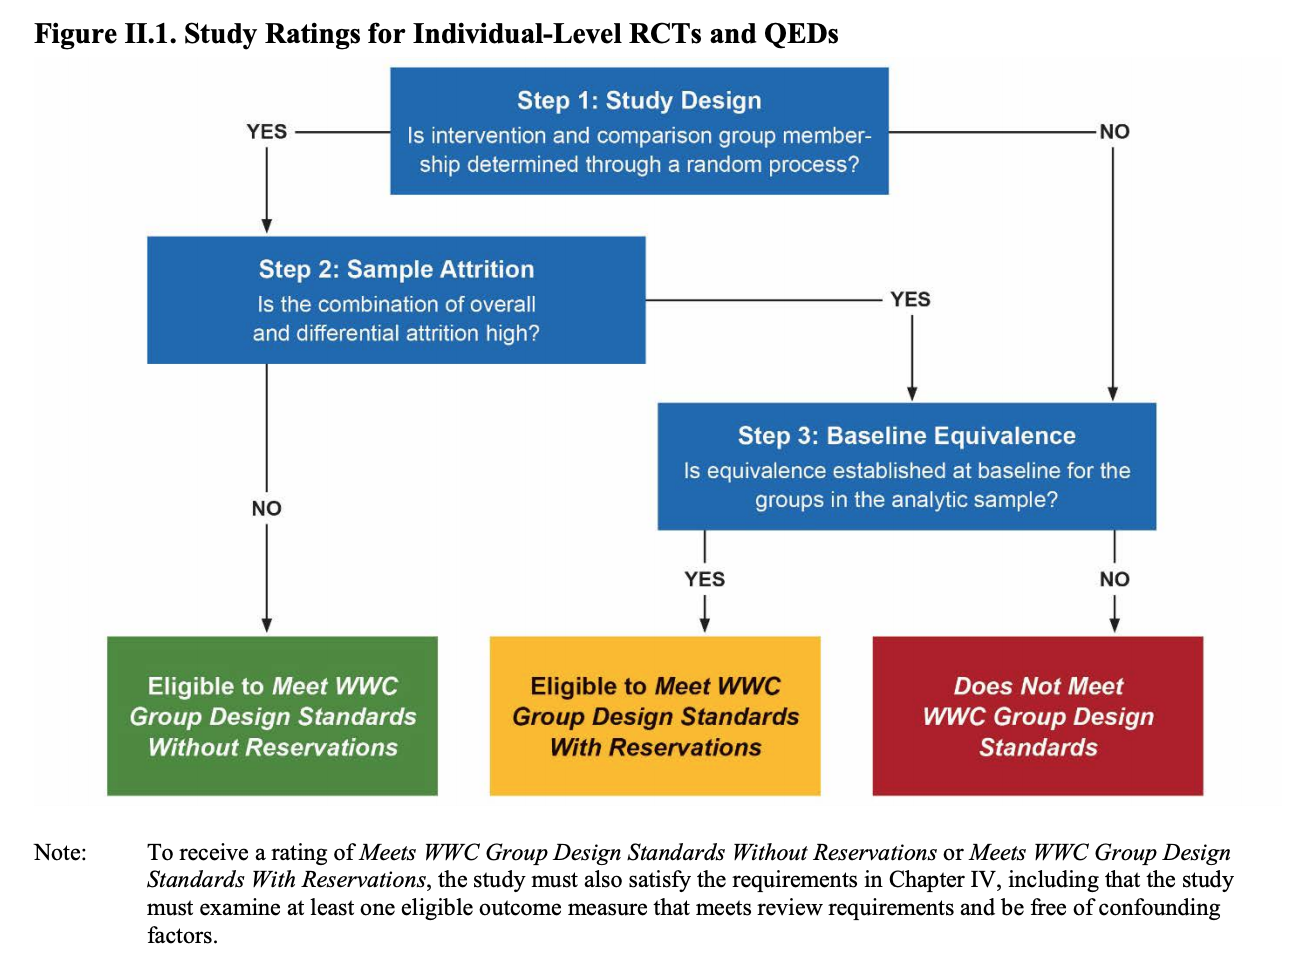
\includegraphics[scale=0.57]{../figs/DoE_standards.png} 
\end{center}


\end{frame}


%%%%%%%%%%%%%%%%%%%%%%%%%%%%%%%%%%%

\section{Design}

\begin{frame}
\frametitle{Overview of experimental design}

\begin{itemize}
\item 2x2 factorial design with two treatments:
\begin{itemize}
\item Evidence standard (low vs. high)
\item Whether evidence standards are explained to policymakers
\end{itemize}
\end{itemize}

\begin{table}[H]
\centering
\caption{Treatment arms: 2x2 factorial design}
\vspace{-7mm}
\label{tab: arms} 
\bigbreak
\begin{tabular}{|l|l|l|l|l|}
\hline
& \textbf{Lower Tier} & \textbf{Higher Tier} \\ \hline
\textbf{No information} & Control & High and no info \\ \hline
\textbf{Information} & Low and info & High and info \\ \hline
\end{tabular}
\end{table}

\end{frame}

%%%%%%%%%%%%%%%%%%%%%%%%%%%%%%%%%%%

\begin{frame}
\frametitle{Power analysis: state}

\only<1>{
\begin{figure}
\vspace{-0.25cm}
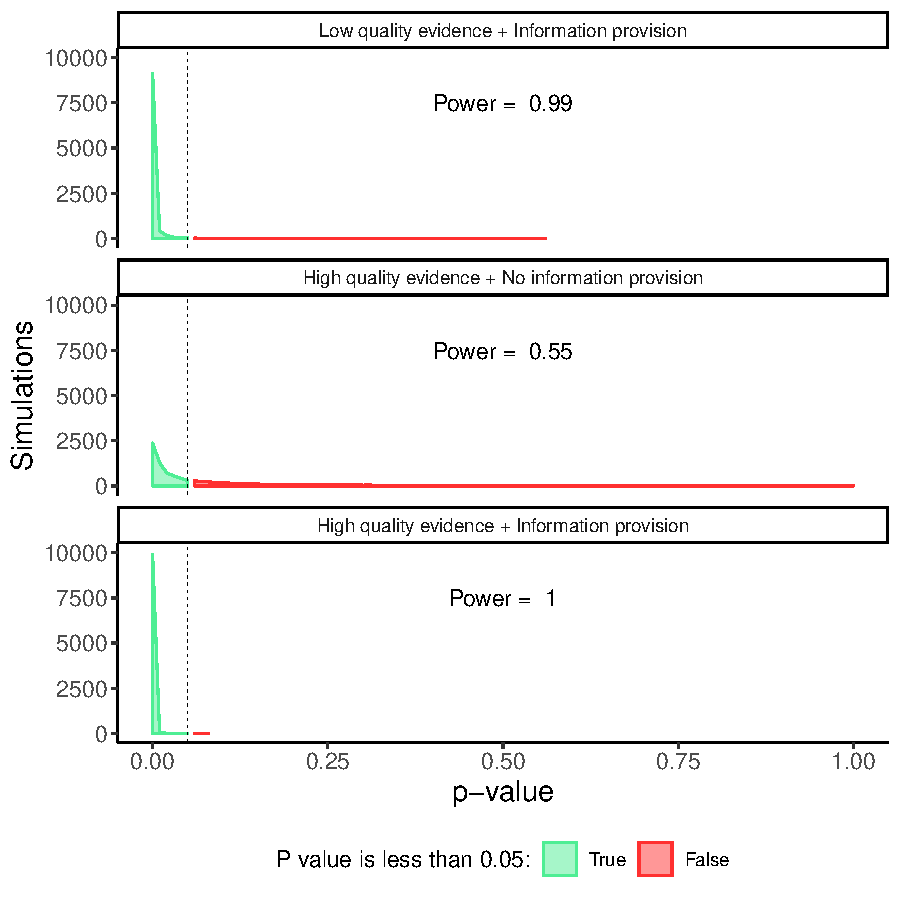
\includegraphics[scale=0.54]{../figs/power_state.pdf}
\end{figure}
}

\end{frame}

%%%%%%%%%%%%%%%%%%%%%%%%%%%%%%%%%%%

\section{Conclusion}

\begin{frame}
\frametitle{Questions}
\begin{itemize}
\item Should we use a neutral or partisan policy proposal?
\begin{itemize}
\item Partisan policy proposal might allow us to test legislator's motivated reason, but power issues.
\end{itemize}
\item Suggestions for kind of organization to partner with?
\item Federal, state, or local level?
\end{itemize}

\end{frame}


%%%%%%%%%%%%%%%%%%%%%%%%%%%%%%%%%%%
\appendix

\section{Supplemental material}

\begin{frame}[label= doe_evidence]
\frametitle{Evidence tiers}

\only<1>{
\begin{figure}
\vspace{-0.25cm}
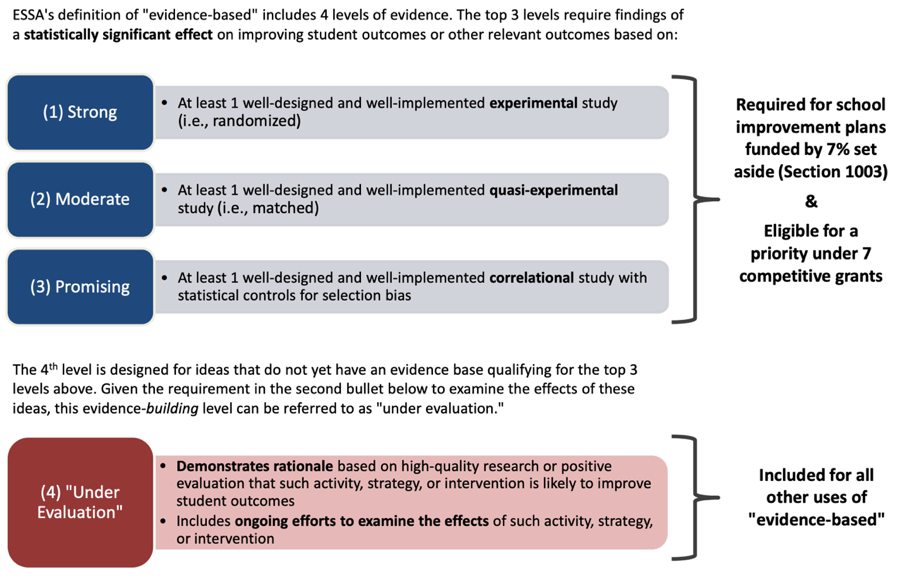
\includegraphics[scale=0.75]{../figs/doe_tiers.png}
\end{figure}
}


\end{frame}


\end{document}